% -----
% COMP2550 proposal
% CHRISTOPHER CLAOUE-LONG
% -----
% -
% - DOCUMENT GEOMETRY SETUP
\documentclass[12pt,a4paper]{article}
\usepackage[margin=20mm]{geometry}
\usepackage{wrapfig}
\usepackage{lastpage} % to display the page number down the bottom
\makeatletter \renewcommand{\@oddfoot}{\hfil Page \thepage\ of \pageref{LastPage} \hfil} \makeatother % Page X of Y down the bottom
% -
% - FONT
\usepackage{amsmath,amsthm,amssymb,graphicx,epstopdf,datetime,multicol,verbatim,ulem,alltt,multirow}
\DeclareGraphicsRule{.tif}{png}{.png}{`convert #1 `dirname #1`/`basename #1 .tif`.png}
\usepackage[sc]{mathpazo} % Palatino maths fonts - acceptable fonts for typesetting, also sets these fonts for use in math mode
\linespread{1.05}
\usepackage[T1]{fontenc}
\usepackage[bitstream-charter]{mathdesign}
% -
% - MISC. PACKAGES
\usepackage[usenames,dvipsnames,svgnames,table]{xcolor}
\usepackage{hyperref}
\hypersetup{
colorlinks,
citecolor=black,		% - Citation colour
filecolor=black,		% - File colour
linkcolor=black,		% - Link colour
urlcolor=black		% - URL colour
}\urlstyle{same}
% -
% -
% - MISC. SYMBOLS AND COMMANDS
\newcommand{\HUGE}[1]{\textbf{\Huge #1}}
\newcommand{\ITALIC}[1]{\textit{#1}}
\newcommand{\BOLDL}[1]{\textbf{\large #1}}
\newcommand{\BOLD}{\textbf}
\newcommand{\Hrule}{\textcolor{blue}{\rule{\linewidth}{0.5mm}}} 

% Defines a new command for the horizontal lines, change thickness here
\newcommand{\htab}{\hspace*{0.63cm}}
\newcommand{\SUPER}{\textsuperscript}
\newenvironment{Figure}
  {\par\medskip\noindent\minipage{\linewidth}}
  {\endminipage\par\medskip}
\newcommand{\TIMELINE}[3]{#1\\\BOLD{#2} #3}
\newcommand{\TIMELINESPACE}{\\[0.3cm]}
% -
% -----
% BEGIN DOCUMENT
% -----
\begin{document}
% -----
% - Title
{\center{\Hrule\vspace{0.2em}
	%
	\HUGE{COMP2550/COMP3130 ANU\\Main Project Proposal}\\
	\BOLDL{
		Christopher Claou\'e-Long
		(\href{mailto:u5183532@anu.edu.au}
		{\ITALIC{\underline{\smash{u5183532@anu.edu.au}}}})\\
		Jimmy Lin 
		(\href{mailto:u5223173@anu.edu.au}
		{\ITALIC{\underline{\smash{u5223173@anu.edu.au}}}})\\
	}
	\BOLD{Last typeset: \currenttime, \today}
\\\Hrule}}
%
% -
\begin{multicols}{2}
\section{Introduction}
\htab A long-standing problem in the field of computer vision is how to calculate the saliency of objects in images, that is the prominence of them compared to the background.  Many approaches exist to attempt to solve this issue, however multiple attemps have either transformed into simple object detection algorithms or are not particularly accurate. 
[needs more on problem motivation, background]\\
% -
% introduce related work 
\htab Today, are a few existing works that achieve a high accuracy in detecting salient objects. The most recognised approach in the last decade is Itti's algorithm from 1998 (see ref.3). It calculates a feature map and then converts it to a rectangle via a winner-take-all algorithm. However, the precision of the detection from this and other algorithms is as yet unsatisfying, even though Itti's algorithm in particular has good object recall. The second approach is the fuzzy-growing approach (see ref.4), which directly outputs a rectangle to label saliency in a less costly way. But its outcome is worse(as shown in the following comparison).
% -
% image outlining salient object detection
\begin{Figure}
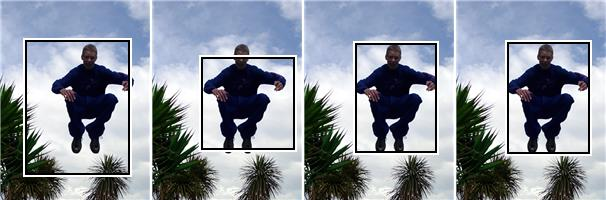
\includegraphics[width=3.2in,height=1in]{./pictures/0_imCanvs_Compare.jpg} \\
{\htab \tiny (a) FG(Ma,2003) (b) SM(Itti,1998) (c) CRFM(Liu,2007) (d) Ground truth}
\end{Figure}
% -
% framework
The research we will be referring to to in this experimental project is that of Liu, Tie et al. in 2011 (see ref.2), which is based on a onditional random field (CRF) model.  This allows a large amount of near-perfect saliency detection compared with the ground truth data. To accomplish this, it extracts features on the local, regional and global level, where it calculates multiscale contrast, a centre-surround histogram and spatial color distribution respectively. After normalization and linear/non-linear combination, a master map, better known as a salient map, is computed to represent the saliency of each image pixel. A few key locations on the saliency map are finally identified by winner-take-all or inhibition-of-return, or other non-linear operations that act on the probability of a salient object being present at the location.
% -
% implementation details
\section{Proposed Implementation}
% implementation outline and explanation of chice
\htab Our implementation will employ the  OpenCV library, leveraging on the ANU's open source DARWIN framework to achieve a CRF-based saliency detection algorithm. The reason for selecting CRF-based saliency detection as our project focus is that this project would give us experience of manipulating graphical model in practice, especially learning and inference mechanism of CRF. Another reason sources from the intuition that this may help scene understanding in multiple ways. For instance, under a complex scene understanding algorithm with dozens of classes label, exclusively labelling the salient region and its near neighbourhood within a tremendously large image saves the computational resources. 
\subsection{Conditional Random Fields}
\htab Conditional Random Fields model the distribution of an objective variable given some ``less global'' factores \BOLDL{EXPAND}.  They can be described by the equation
    $$ P(A|I) = \frac{1}{Z} \cdot\exp(-E(A|I)) $$
where $E(A|I)$ is the energy function, formulated to be a set of static salient features and one pairwise feature as follows:
    $$ E(A|I) = \sum_{x} \sum_{k=1}^{K} \lambda_{k} F_{k}(a_{x},I)  
        + \sum_{x,x'} S(a_{x},a_{x'},I)  $$ \vspace{-0.4cm}
\begin{center} \footnotesize $\lambda_{k}$: weight of $k$th feature, $x,x'$: two adjacent pixels. \end{center} 
%
\subsection{Feature Extraction Ideas}
\textbf{Multiscale Contrast}. This static feature extracts intensity, color, orientation, texture at multiple scales to capture hight contrast in the boundary of objects . \\[0.1cm]
\textbf{Center-Surround Histogram}. This static feature can be computed using various low-level features by a center-surround operation.  \\[0.1cm]
\textbf{Spatial Color distribution}. This static feature penalizes the pixels with widely distributed color. \\[0.1cm]
\textbf{Pairwise Feature}. This feature exploits the spatial relationship between two adjacent pixels and can be viewed as one capturing the spatial continuity of saliency, that is, adjacent pixels that are prone to be assigned with different labels. 
\subsection{Possible Improvements}
\htab First and foremost, one possible breakthrough lies in enhancing the quality of extracted features for detecting sliency. From the result presentation of referred approach (Tie, ref.2), the saliency of legs of animals (i.e. horses, elk) are frequently missed even in the feature map. Perhaps this is because of the thinness of the legs.
\section{Project Timeline}
\TIMELINE{1\SUPER{st}  - 18\SUPER{th} April}{Project Proposal:}{Research current literature to find papers and inspire a project of interest, determine the topic of our second project and collect relevant datasets for training.}\TIMELINESPACE
%
\TIMELINE{19\SUPER{th} April - 28\SUPER{th} April}{Framework Construction:}{Gain familiarity with the packages and existing frameworks and implementations in Darwin and OpenCV, set up the interface to accept training data and the CRF model for saliency learning and inference.} \TIMELINESPACE
%
\TIMELINE{29\SUPER{th} April - 12\SUPER{th} May}{Implementation:}{Design and implement algorithms to calculate various features and output a rectangle/rectangles labeling the salient object(s).}\TIMELINESPACE
%
\TIMELINE{12\SUPER{th} May- 19\SUPER{th} May}{Testing and Improvements:}{Test the framework, review or research possible improvements and implmenent.}\TIMELINESPACE
%
\TIMELINE{20\SUPER{th} May - 30\SUPER{th} May}{Project Review and Report:}{Write up report summarising our project and findings, prepare presentation.}
% References
\begin{thebibliography}{0} \footnotesize   \setlength{\itemsep}{-0.5pt}%
    \bibitem 1 Gould, Stephen. "DARWIN: A Framework for Machine Learning and Computer Vision Research and Development." \textit{Journal of Machine Learning Research 13 (2012): 3533-3537}. 
    \bibitem 2 Liu, Tie, et al. "Learning to detect a salient object." \textit{Pattern Analysis and Machine Intelligence, IEEE Transactions on 33.2 (2011): 353-367}. 
    \bibitem 3 Itti, Laurent, Christof Koch, and Ernst Niebur. "A model of saliency-based visual attention for rapid scene analysis."\textit{ Pattern Analysis and Machine Intelligence, IEEE Transactions on 20.11 (1998): 1254-1259}.
    \bibitem 4 Ma, Yu-Fei, and Hong-Jiang Zhang. "Contrast-based image attention analysis by using fuzzy growing."\textit{ Proceedings of the eleventh ACM international conference on Multimedia. ACM, 2003}. 
\end{thebibliography}
\end{multicols}
\vfill\Hrule
\end{document}
% -----
% END OF LINE
% -----
